\documentclass[a4paper,11pt]{report}
\usepackage[utf8]{inputenc}  
\usepackage[italian]{babel}
\usepackage{indentfirst}
\usepackage{tocloft}
\renewcommand{\cftchapdotsep}{\cftdotsep}
\raggedbottom
\usepackage{epigraph}
\usepackage[T1]{fontenc}        % include i font in maniera vettoriale azichè 
\usepackage{lmodern}            % latin modern fonts
\usepackage{graphicx,color}     % per le immagini
\usepackage{latexsym}           
\usepackage{setspace}          
\usepackage{amsmath}            % package per la matematica
\usepackage{amsfonts}           % idem
\usepackage{amssymb}            % idem
\usepackage{amsthm}             % idem
\usepackage{fancyvrb}           % package per il comando VerbatimInput
\usepackage{hyperref}
\usepackage{listings}
\usepackage{lettrine}

\lstset{language = Java, numbers = left, basicstyle=\footnotesize, numberstyle=\footnotesize,tabsize=2}

%Da sistemare con l'icona del programma.
\title{\textbf{Progetto \newline Laboratorio Programmazione di rete \newline Mini-KaZaA}}
\author{Andrea Di Grazia, Massimiliano Giovine
                }
\date{Anno Accademico 2008 - 2009}

\begin{document}
\maketitle
\tableofcontents

%Introduzione al progetto
\input{introduzione.tex}
%Spiegazione implementazione del bootstrap server
\chapter{Bootstrap Server}

Il bootstrap server si avvia dal main situato all'interno del file \verb|BootstrapService.java|. Questo file esegue subito un blocco di tipo \verb|try{}catch| nel quale si trovano le seguenti istruzioni.

\begin{lstlisting}

\end{lstlisting}
%Spiegazione implementazione del client della rete mini-kazaa
\chapter{Mini-KaZaA Client}
Oltre che di un Bootstrap server, la rete Mini-KaZaA si basa su un client che gli utenti possono usare per accedere alla rete e poter condividere e scaricare file.
\section{Mini-KaZaA Client in generale}
Mini-KaZaA client presenta tutte le funzionalità che consentono una condivisione peer to peer dei contenuti.
Ogni client al primo avvio chiede all'utente, tramite un comodo pannello, di scegliere il \emph{ruolo} da interpretare all'interno della rete.

Chi ha più risorse da mettere a disposizione e una banda di comunicazione più ampia può scegliere di essere un Super Node, che oltre a condividere e scaricare, ha la funzione di smistare le query nella rete e accettare richieste direttamente dagli Ordinary Node \emph{figli}. Chi ha meno risorse da mettere a disposizione può scegliere di essere un semplice Ordinary Node.

\section{Il codice di Mini-KaZaA client}
Il codice di Mini-KaZaA client è distribuito in tre diverse librerie:
\begin{itemize}
 \item \textbf{lpr.minikazaa.minikazaaclient}: questa libreria contiene classi comuni a tutti e due i tipi di client dal punto di vista logico. L'esempio più evidente è la classe \verb|MainGui.java|.
 \item \textbf{lpr.minikazaa.minikazaaclient.ordinarynode}: questa libreria contiene le classi che loogicamente appartengono al tipo di client Ordinary Node, ma che, all'occorrenza, possono essere importate anche da un Super Node.
 \item \textbf{lpr.minikazaa.minikazaaclent.supernode}: questa libreria, infine contiene tutte le classi che servono a un supernodo per funzionare e che appartengono a questo logicamente. Alcune di queste classi, come per esempio \verb|SupernodeCallbacksInterface.java|, vengono utilizzate anche dagli ORdinary Node.
\end{itemize}

Questa suddivisione è puramente logica visto che i due tipi di client differiscono solo per alcune caratteristiche.

Si è preferito dividere anche le classi che contengono gli stessi task per i SN e per gli ON per poter meglio gestire il codice e renderlo più modulare.
Un esempio è rappresentato dalle classi \verb|OrdinarynodeWorkingThread.java| e \verb|SupernodeWorkingThread.java| che hanno lo stesso compito, ma, che piuttosto che complicare con una serie di 
\begin{verbatim}
if <condizione> then 
	<blocco> 
else 
	<blocco>|
\end{verbatim}
si è preferito separare in due classi distinte.

Passiamo ora a una presentazione più particolareggiata del codice comune a Super Node e Ordinary Node.

\section{Le strutture dati comuni}
Per lo sviluppo di Mini-KaZaA è stato necessario predisporre una serie di strutture dati che tutto il software
utilizzi per condividere informazioni.

All'interno del package \verb|lpr.minikazaa.minikazaaclient| troviamo le seguenti classi che rappresentano strutture dati comuni a SN e ON:
\begin{itemize}
 \item \verb|NodeConfig.java|
 \item \verb|Query.java|
 \item \verb|Answer.java|
 \item \verb|SearchField.java|
 \item \verb|Download.java|
 \item \verb|DownloadRequest.java|
 \item \verb|DownloadResponse.java|
\end{itemize}

Guardiamo cosa si nasconde all'interno di ognuna di queste classi.

\subsection{NodeConfig.java}
La classe \verb|NodeConfig.java| contiene i seguenti attributi:
\newline
\begin{lstlisting}
private String user_name;
private int port;
private String bootstrap_address;
private int max_conn;
private int ttl;
private boolean is_sn;

//Calcolato all'avvio
private String my_address;
\end{lstlisting}

Questi attributi sono i campi che l'utente inserisce nel form al primo avvio del programma e contengono le informazioni di configurazione del nodo. 

\subsection{Query.java}
La classe \verb|Query.java| viene utilizzata dal client Mini-KaZaA per l'invio di richieste di file nella rete.

Contiene diversi attributi per i quali ci sono i metodi \verb|set| e \verb|get|. Questa classe inoltre implementa
le interfacce \verb|Serializable| e \verb|Cloneable|.
La prima serve per poter inviare su rete come flusso di byte l'oggetto \verb|Query|. La seconda invece serve per poter
copiare un'istanza dell'oggetto \verb|Query| in una seconda istanza.
\newline
\begin{lstlisting}
private String body_q;              //Regex of a sended query
private Answer body_a;              //Answer query
private OrdinarynodeFiles body_f;   //Notify a supernode to 
                                 	//have many files to share.
private NodeInfo id_origin;         //Source of a query
private NodeInfo sender;            //NodeInfo of sender node.
private NodeInfo receiver;          //NodeInfo of receiver node

private int ttl;                    //Time to live of a query
private int id;                     //Id of origin query
\end{lstlisting}

La classe \verb|Query| ha tre gruppi di attributi.Un primo gruppo descrive il contenuto della query e di conseguenza
il tipo di query. Un secondo gruppo serve per identificare i soggetti coinvolti nello scambio della query stessa.
Il terzo gruppo contiene invece parametri per l'identificazione della query. 

Analizziamo uno ad uno questi parametri per capire meglio come funzionano le query in Mini-KaZaA.
\begin{itemize}
 \item \verb|body_q|:
il vero corpo della query di richiesta di un file. \`{E} una stringa che contiene un
espressione regolare che il client Mini-KaZaA riesce a interpretare;

 \item \verb|body_a|:
la parte dell'oggetto \verb|Query| che contiene la risposta a una determinata richiesta. Analizzaremo la classe
\verb|Answer| successivamente;

 \item \verb|body_f|:
questo campo viene riempito da un ON che vuole inviare al proprio SN la sua lista di file per metterli a disposizione
di tutti;

 \item \verb|id_origin|:
per ogni query deve essere nota l'origine dalla quale proviene la query stessa per poi poterla correttamente fermare
al punto giusto e farla ritornare al mittente. Questo è il compito del campo \verb|id_origin|;

 \item \verb|sender|: 
questo campo indica uno dei due soggetti che sono impegnati in un singolo scambio di query, il nodo da cui parte;

 \item \verb|receiver|:
questo campo indica il nodo a cui deve arrivare la query in uno scambio;

 \item \verb|ttl|:
questo campo sta per \emph{Time To Live} e indica il numero di scambi per il quale la query deve continuare a esistere.
Serve principalmente per evitare che si creino dei cicli infiniti di scambio della query ottenendo quindi una valanga
di dati ridondanti con conseguente intasamento della rete;

 \item \verb|id|:
ogni nodo può inviare più query alla volta nella rete e il compito di questo campo è di identificare univocamente la
query presso il suo nodo origine.
\end{itemize}

\subsection{Answer.java}
La classe \verb|Answer.java| contiene i file che possono corrispondere ai criteri di una ricerca. 

\`{E} una classe molto semplice ma molto utile per indicizzare rapidamente i file.

Ecco il codice nel quale vengono dichiarati gli attributi della classe.
\newline
\begin{lstlisting}
//List of files that corresponding to a query.
private ArrayList <OrdinarynodeFiles> files;

//Id of origin query
private int id;
\end{lstlisting}

L'attributo \verb|files| è una lista di OrdinarynodeFiles, Sezione \ref{sec:on_files}.

La classe \verb|Answer.java| viene utilizzata 

L'attributo \verb|id| richiama semplicemente l'id univoco della query di cui fa parte l'oggetto \verb|Answer|.

\subsection{SearchField.java}
La classe \verb|SearchField.java| viene utilizzata dal client Mini-KaZaA per tenere in memoria tutti i risultati
associati a una richesta di file.
Da uno di questi campi poi vengono estratte le informazioni per eventuali download di file.

Anche questa classe è piuttosto semplice poichè funziona da appoggio alla rappresentazione grafica e per snellire
la quantità di informazioni da tenere in memoria per l'utente.

Il codice che descrive gli attributi della classe è il seguente:
\newline
\begin{lstlisting}
//File owner
private NodeInfo owner;

//File descriptor
private MKFileDescriptor file;
\end{lstlisting}

Con queste due semplici informazioni è possibile sia risalire al proprietario, compreso l'indirizzo ip da contattare
per il download, sia ottenere tutti i metadati del file da scaricare\footnote{I download così come le ricerche vengono
effettuati mediante l'hash univoco md5 che tratteremo nella Sezione \ref{sec:md5}}.

\subsection{Download.java}

\subsection{DownloadRequest.java}
\subsection{DownloadResponse.java}

\section{Il percorso di una query}
\section{La grafica del client Mini-KaZaA}
\begin{figure}[t]
 \centering
 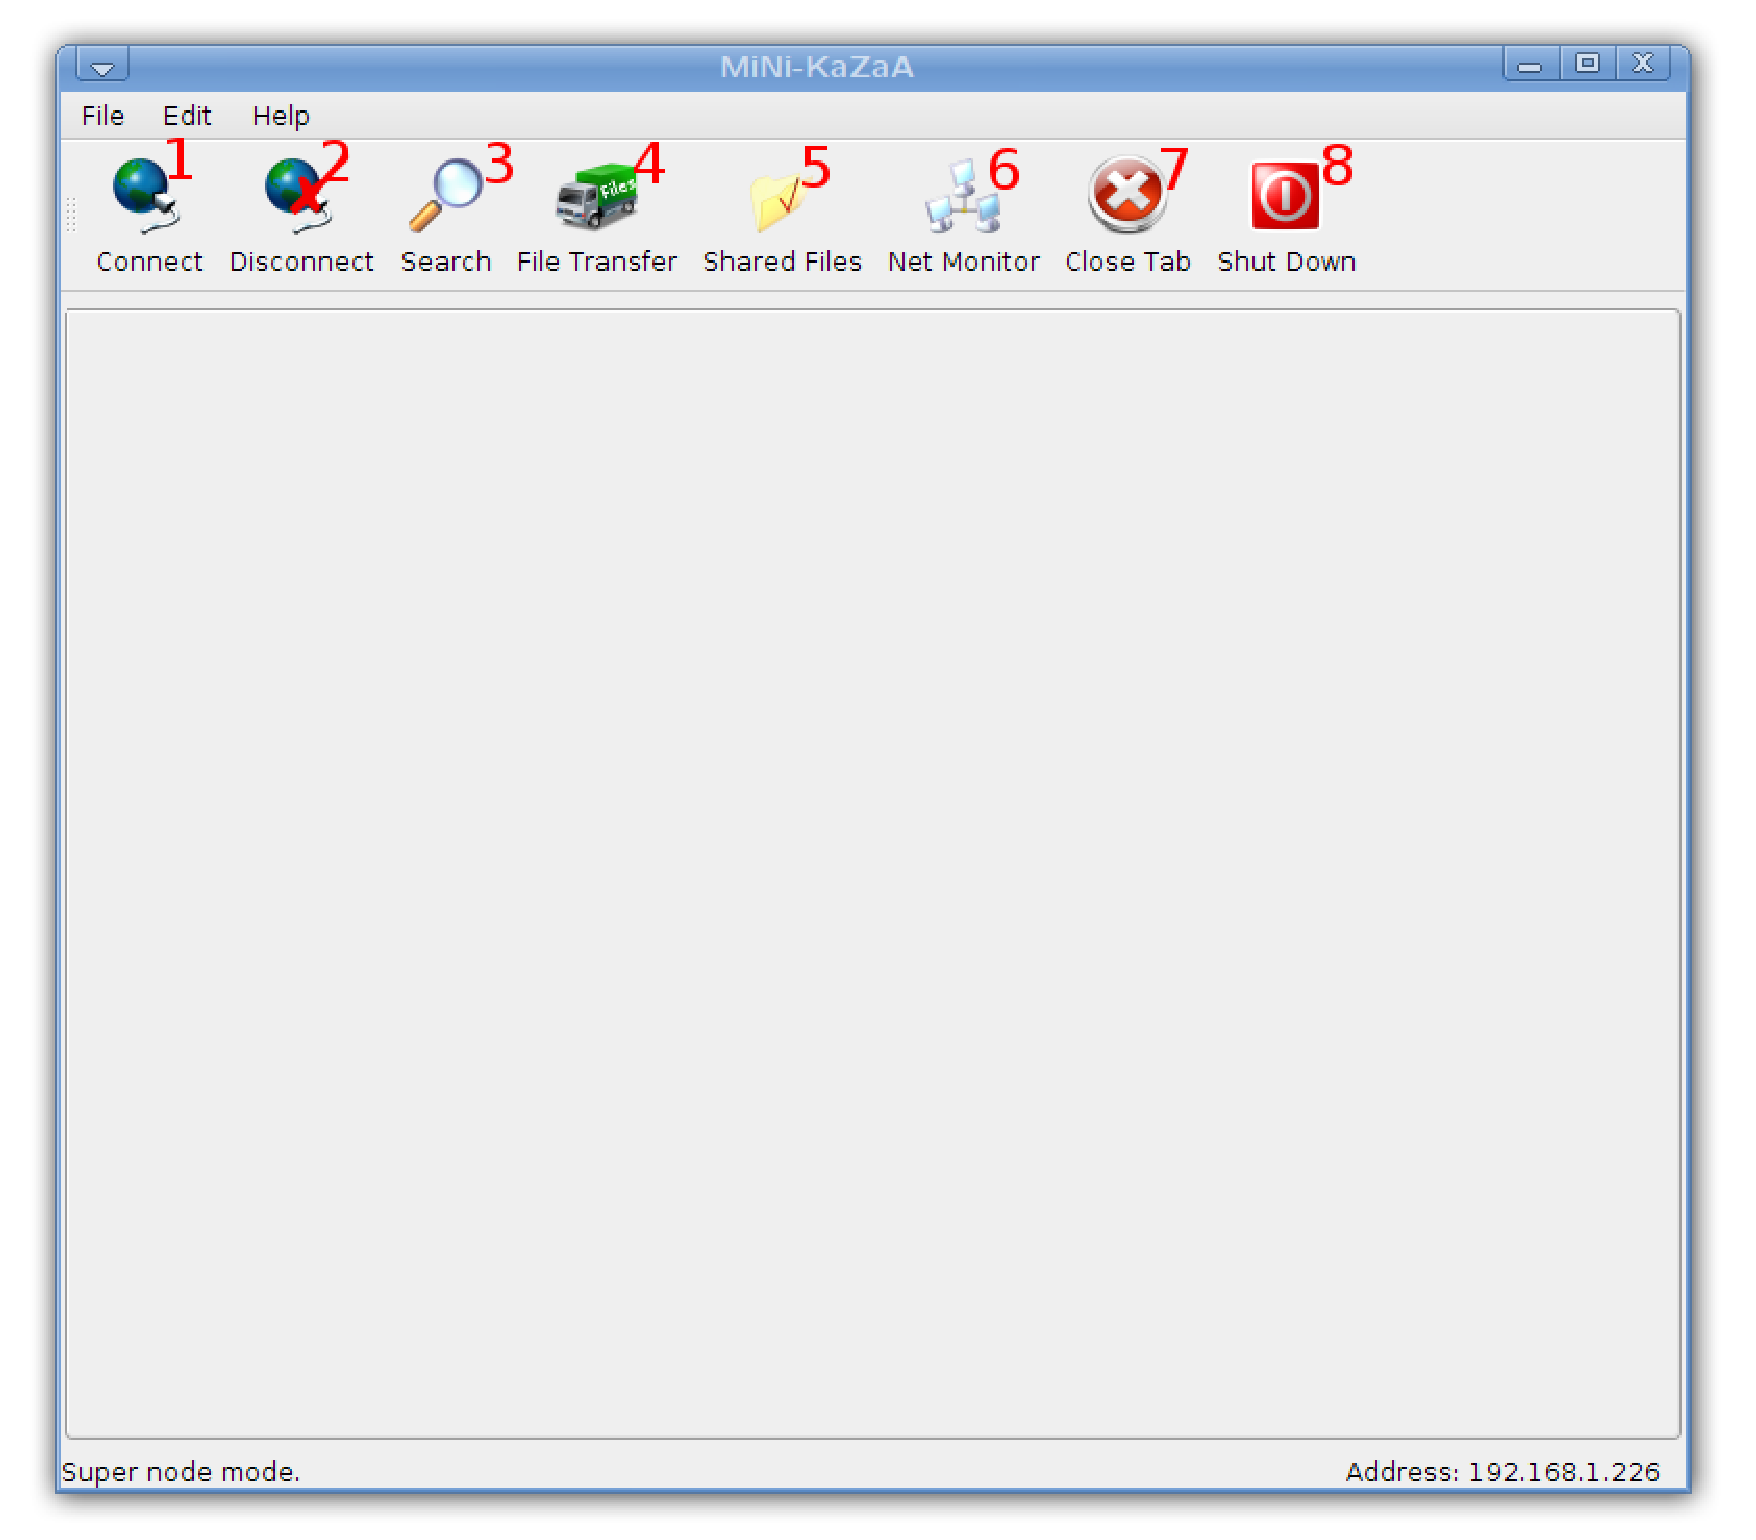
\includegraphics[width=250px,height=225px,bb=14 14 841 737]{images/mini_kazaa_client.eps}
 % mini_kazaa_client.eps: 0x0 pixel, 300dpi, 0.00x0.00 cm, bb=14 14 841 737
 \caption{L'interfaccia grafica principale del client.}
 \label{fig:mini_kazaa_client}
\end{figure}


%Spiegazione implementazione delle peculiarità dell'ordinary node
\chapter{Ordinary Node}
\section{Le classi del package lpr.minikazaaclient.ordinarynode}
\subsection{OrdinarynodeFiles.java}\label{sec:on_files}

\section{Scelta del SN al quale connettersi}\label{sec:scelta_sn}
\section{Lo scambio di file}\label{sec:scambio}
\section{Condivisione di file}
La condivisione di file avviene non appena l'utente di un ON decide di condividere file tramite l'apposito pannello descritto in Sezione \ref{sec:grafica}

%Spiegazione implementazione delle peculiarità del super node
\chapter{Super Node}
\section{L'interfaccia per le callback}
%Descrizione package di utilità
\chapter{Il package Util}
\section{Calcolo dell'md5}\label{sec:md5}
%Una descrizione dettagliata del package contenente le classi 
%per la grafica
\chapter{Il package di grafica}
\chapter{Scelte di progetto e cenni di teoria}\label{chap:scelte_di_progetto}

\section{Java Bean}\label{sec:java_bean}
Le JavaBean sono usate per incapsulare molti oggetti in un singolo oggetto (il bean), così da poter passare il bean invece degli oggetti individuali.
Al fine di funzionare come una classe JavaBean, una classe comune di un oggetto deve obbedire a certe convenzioni in merito ai nomi, alla costruzione e al comportamento dei metodi. 
Le convenzioni richieste sono:
\begin{itemize}
    \item La classe deve avere un costruttore senza argomenti.
    \item Le sue proprietà devono essere accessibili usando get, set e altri metodi (così detti metodi accessori).
    \item La classe dovrebbe essere serializzabile (capace di salvare e ripristinare il suo stato in modo persistente).
    \item Non dovrebbe contenere alcun metodo richiesto per la gestione degli eventi.
\end{itemize}

Utilizzando queste proprietà, i Java Bean sono risultati molto utili sia per creare strutture facilmente inviabili via rete, sia per utilizzare le classi XMLEncoder e XMLDecoder per scrivere e leggere Java Bean da file XML.

\section{UML Logica}\label{sec:UML_logica}
\begin{figure}[t]
 \centering
 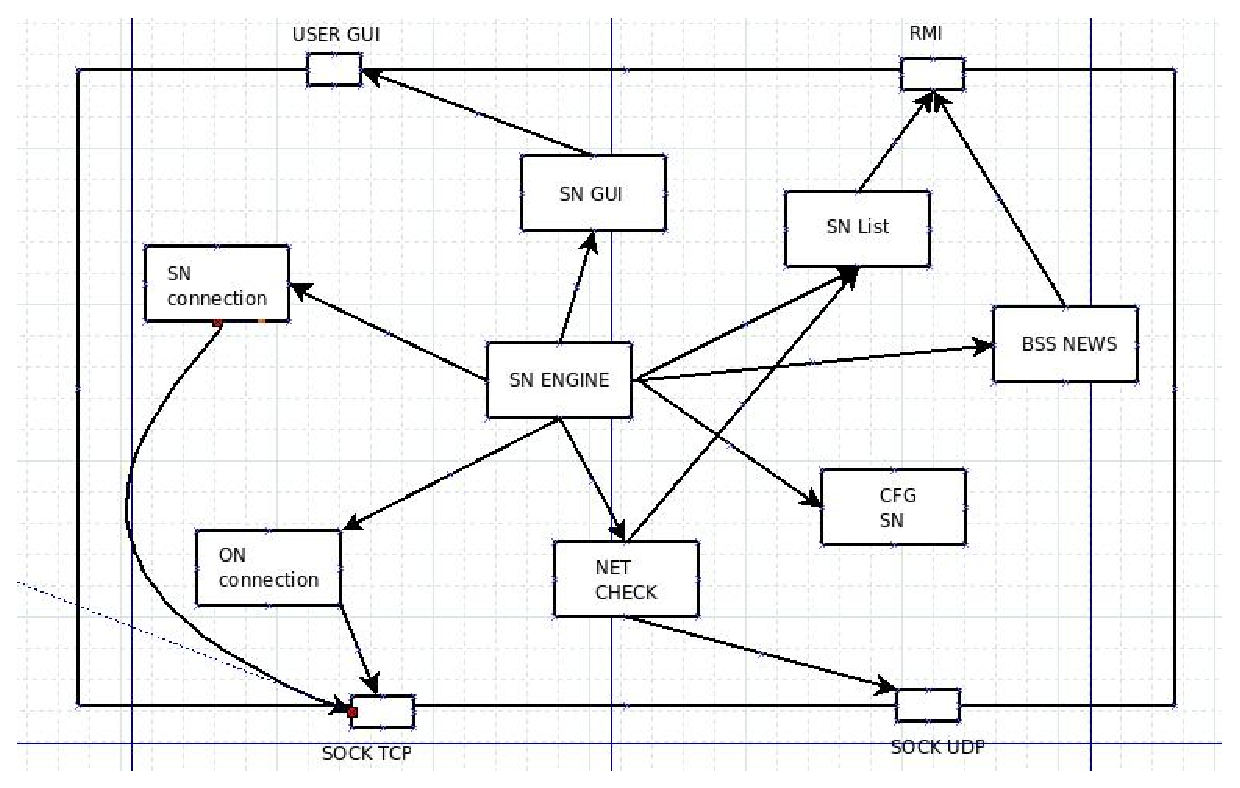
\includegraphics[width=400px,height=225px,bb=14 14 593 376]{images/logica_uml.eps}
 % logica_uml.eps: 0x0 pixel, 300dpi, 0.00x0.00 cm, bb=14 14 593 376
 \caption{Il diagramma UML che rappresenta la logica di Mini-KaZaA.}
 \label{fig:logica_uml}
\end{figure}
%Inserire una breve descrizione del diagramma UML
La logica del programma è visualizzabile in Figura \ref{fig:logica_uml}.
Il diagramma UML si riferisce un nodo di tipo SN, ma, visto che possiamo considerare i SN come degli ON con alcune funzionalità in più, questo diagramma vale anche per gli ON.

Possiamo vedere come ogni nodo abbia due tipi di componenti:
\begin{itemize}
 \item componenti logica interna;
 \item componenti di interfaccia con il mondo esterno.
\end{itemize}

Tutti questi componenti vengono gestiti da un motore centrale che richiama opportunamente le strutture dati utilizzate e i thread che devono svolgere i vari compiti.


\section{Classe Wrapper per il socket}\label{sec:wrap_sock}
Il fine del Wrapper è di fornire una soluzione astratta al problema dell'interoperabilità tra interfacce differenti. Il problema si presenta ogni qual volta nel progetto di un software si debbano utilizzare sistemi di supporto (come per esempio librerie) dotati di interfaccia non perfettamente compatibile con quelle richieste da applicazioni già esistenti. Invece di dover riscrivere parte del sistema, oneroso e non sempre possibile se non si ha a disposizione il codice sorgente, può essere comodo scrivere un Adapter che faccia da tramite tra le diverse interfacce, rendendole così compatibili.

Il wrapper inoltre ci ha consentito di poter inizializzare un oggetto che ci serviva all'interno di un \emph{sotto-thread} all'interno dell'\emph{engine} per poi modificarne il contenuto all'interno dei vari sotto-thread non appena si rendevano disponibili le informazioni per completarne la struttura.


\section{Il protocollo  TCP}
Il TCP nacque nel 1970 come frutto del lavoro di un gruppo di ricerca del dipartimento di difesa statunitense. I suoi punti di forza sono l'alta affidabilità e robustezza.
Il protocollo TCP serve a creare degli stream socket, cioè una forma di canale di comunicazione che stabilisce una connessione stabile fra due stazioni, in modo che queste possano scambiarsi dei dati.

Il servizio offerto da TCP è il trasporto di un flusso di byte bidirezionale tra due applicazioni in esecuzione su host differenti. Il protocollo permette alle due applicazioni di trasmettere contemporaneamente nelle due direzioni, quindi il servizio può essere considerato "Full Duplex" anche se non tutti i protocolli applicativi basati su TCP utilizzano questa possibilità.
Il flusso di byte viene frazionato in blocchi per la trasmissione dall'applicazione a TCP (che normalmente è implementato all'interno del sistema operativo), per la trasmissione all'interno di segmenti TCP, per la consegna all'applicazione che lo riceve, ma questa divisione in blocchi non è per forza la stessa nei diversi passaggi.
TCP è un protocollo orientato alla connessione, ovvero prima di poter trasmettere dati deve stabilire la comunicazione, negoziando una connessione tra mittente e destinatario, che viene esplicitamente chiusa quando non più necessaria. Esso quindi ha le funzionalità per creare, mantenere e chiudere una connessione.
TCP garantisce che i dati trasmessi, se giungono a destinazione, lo facciano in ordine e una volta sola. Questo è realizzato attraverso vari meccanismi di acknowledgment e di ritrasmissione su timeout.
TCP possiede funzionalità di controllo di flusso e di controllo della congestione sulla connessione, attraverso il meccanismo della finestra scorrevole. Questo permette di ottimizzare l'utilizzo della rete anche in caso di congestione.

\section{Il protocollo UDP}
A differenza del TCP, l'UDP è un protocollo di tipo connectionless, inoltre non gestisce il riordinamento dei pacchetti né la ritrasmissione di quelli persi, ed è perciò generalmente considerato di minore affidabilità. È in compenso molto rapido ed efficiente per le applicazioni "leggere" o time-sensitive. Ad esempio, è usato spesso per la trasmissione di informazioni audio o video. Dato che le applicazioni in tempo reale spesso richiedono un ritmo minimo di spedizione, non vogliono ritardare eccessivamente la trasmissione dei pacchetti e possono tollerare qualche perdita di dati, il modello di servizio TCP può non essere particolarmente adatto alle loro caratteristiche. L'UDP fornisce soltanto i servizi basilari del livello di trasporto, ovvero:
\begin{itemize}
    \item multiplazione delle connessioni, ottenuta attraverso il meccanismo delle porte
    \item verifica degli errori mediante una checksum, inserita in un campo dell'intestazione del pacchetto.
\end{itemize}
mentre TCP garantisce anche il trasferimento affidabile dei dati, il controllo di flusso e il controllo della congestione.
L'UDP non tiene nota dello stato della connessione, dunque ha rispetto al TCP informazioni in meno da memorizzare. Un server dedicato ad una particolare applicazione che scelga UDP come protocollo di trasporto può supportare molti più client attivi.

\section{Remote Method Invocation}
In informatica, e in particolare nel contesto del linguaggio di programmazione object-oriented Java, Remote Method Invocation (invocazione remota di metodi) o RMI è una tecnologia che consente a processi Java distribuiti di comunicare attraverso una rete. Questa tecnologia include una API (application programming interface) il cui scopo esplicito è quello di rendere trasparenti al programmatore quasi tutti i dettagli della comunicazione su rete. Essa consente infatti di invocare un metodo di un oggetto remoto (cioè appartenente a un diverso processo, potenzialmente su una diversa macchina) quasi come se tale oggetto fosse "locale" (ovvero appartenente allo stesso processo in cui viene eseguita l'invocazione). In questo senso, la tecnologia RMI può essere ricondotta, da un punto di vista concettuale, all'idea di chiamata di procedura remota riformulata per il paradigma object-oriented (in cui, appunto, le procedure sono sostituite da metodi).
L'utilizzo di un meccanismo di invocazione remota di metodi in un sistema object-oriented comporta notevoli vantaggi di omogeneità e simmetria nel progetto, poiché consente di modellare le interazioni fra processi distribuiti usando lo stesso strumento concettuale che si utilizza per rappresentare le interazioni fra i diversi oggetti di una applicazione, ovvero la chiamata di metodo. 

\section{Utilizzo dei ThreadPool}\label{sec:thread_pool}
In molte applicazioni vengono creati thread il cui stato è quasi sempre sospeso, in attesa che si verifichi un evento. Altri thread potrebbero entrare in uno stato di inattività ed essere attivati solo periodicamente alla ricerca di informazioni sullo stato di una modifica o di un aggiornamento. Il polling del thread consente di utilizzare i thread in modo più efficiente fornendo all'applicazione un pool di thread di lavoro gestiti dal sistema. Un unico thread consente di controllare lo stato di varie operazioni di attesa in coda nel pool di thread. Quando un'operazione di attesa viene completata, la funzione di callback corrispondente viene eseguita da un thread di lavoro contenuto nel pool di thread.

\section{Come funzionano le query}\label{sec:risposte_vuote}
Per aiutare a comprendere il meccanismo che stà dietro al nostro sistema di comunicazione per la ricerca di un file abbiamo creato una semplice vignetta che facilita il tutto.
\begin{figure}[t]
 \centering
 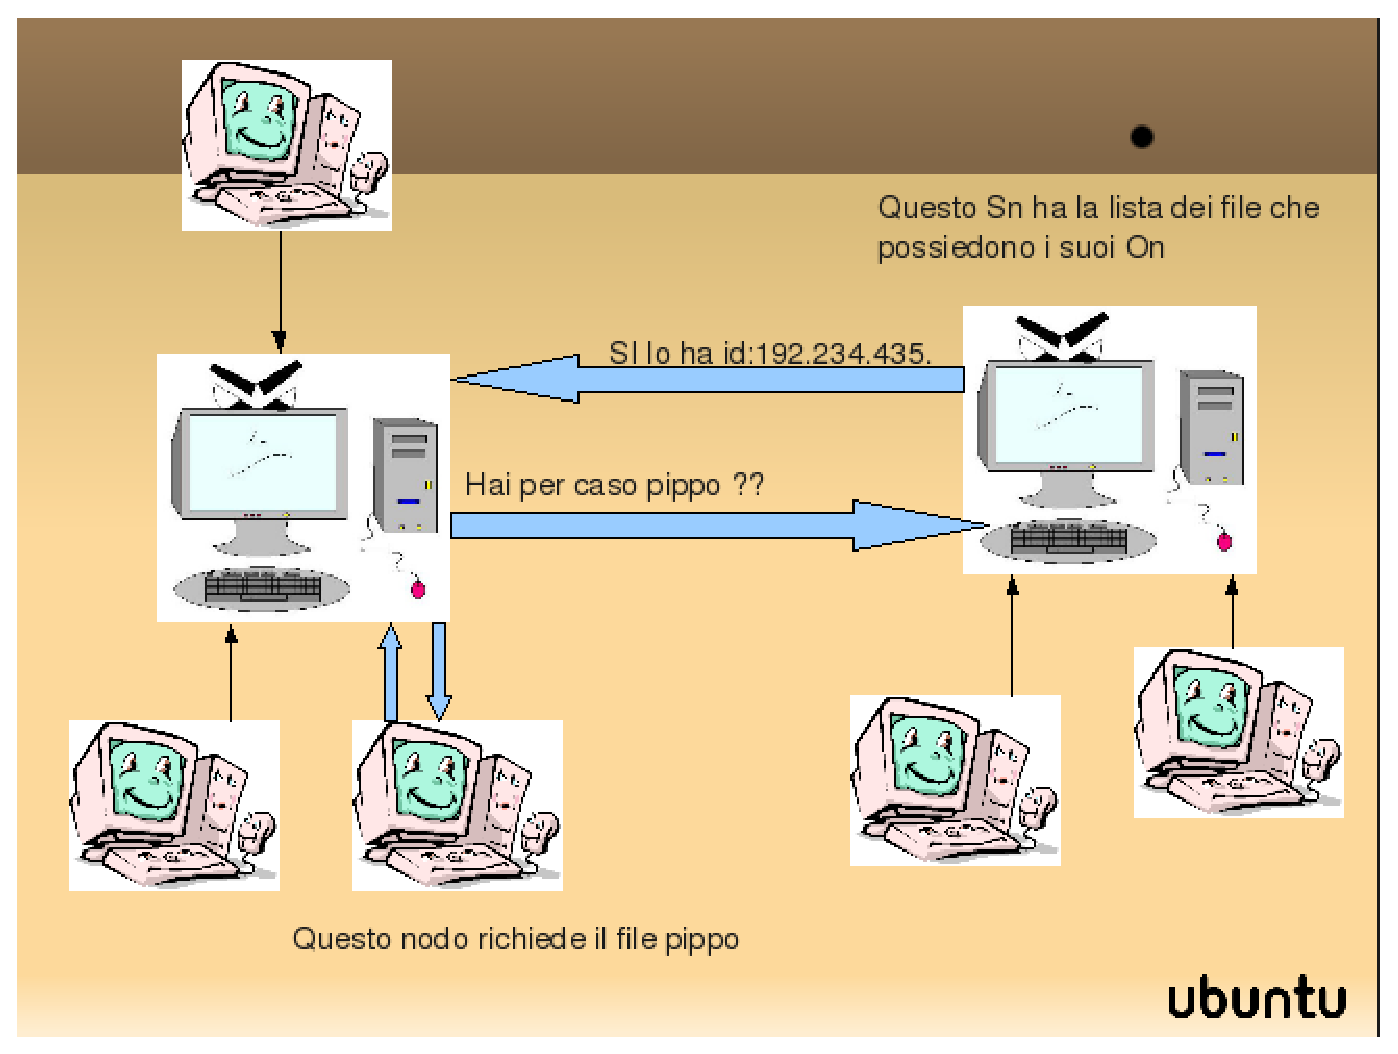
\includegraphics[width=400px,height=375px,bb=14 14 841 737]{images/pippo.eps}
 % mini_kazaa_client.eps: 0x0 pixel, 300dpi, 0.00x0.00 cm, bb=14 14 841 737
 \caption{Richiesta file.}
 \label{fig:richiesta_file}
\end{figure}
Analiziamo insieme come avvengono le comunicazioni.
Come possiamo notare dalla prima figura un utente che ricerca un file effettua la richiesta al SuperNode al quale � connesso direttamente. 
Il SuperNode possiede la lista di tutti i file in possesso dei suoi OrdinaryNode, se il file richiesto appartiene a quelli in suo possesso risponde al mittente con l' indirizzo del nodo che possiede in file.
Se non lo possiede invece chiede agli altri SuperNode ai quali lui � collegato nella rete e attende la risponsta.
La risposta che gli viene data comprende oltre a bit di controllo inseriti dai programmatori per verificare che la query che ritorna sia quella giusta e non una che abbia sbagliato percorso nella rete, l' indirizzo del nodo che possiede il file. Tale risposta viene girata al nodo che inizialmente ha richiesto il file.
A questo punto come viene mostrato nella seconda figura avviene la comunicazione diretta tra il richiedente ed il possessore del file. Comunicazione che avviene tramite un protocollo TCP.
Interessante sottolineare che � stata rispettata la richiesta del testo di avere un percorso a ritroso delle query dal mittente al destinatario.
\begin{figure}[t]
 \centering
 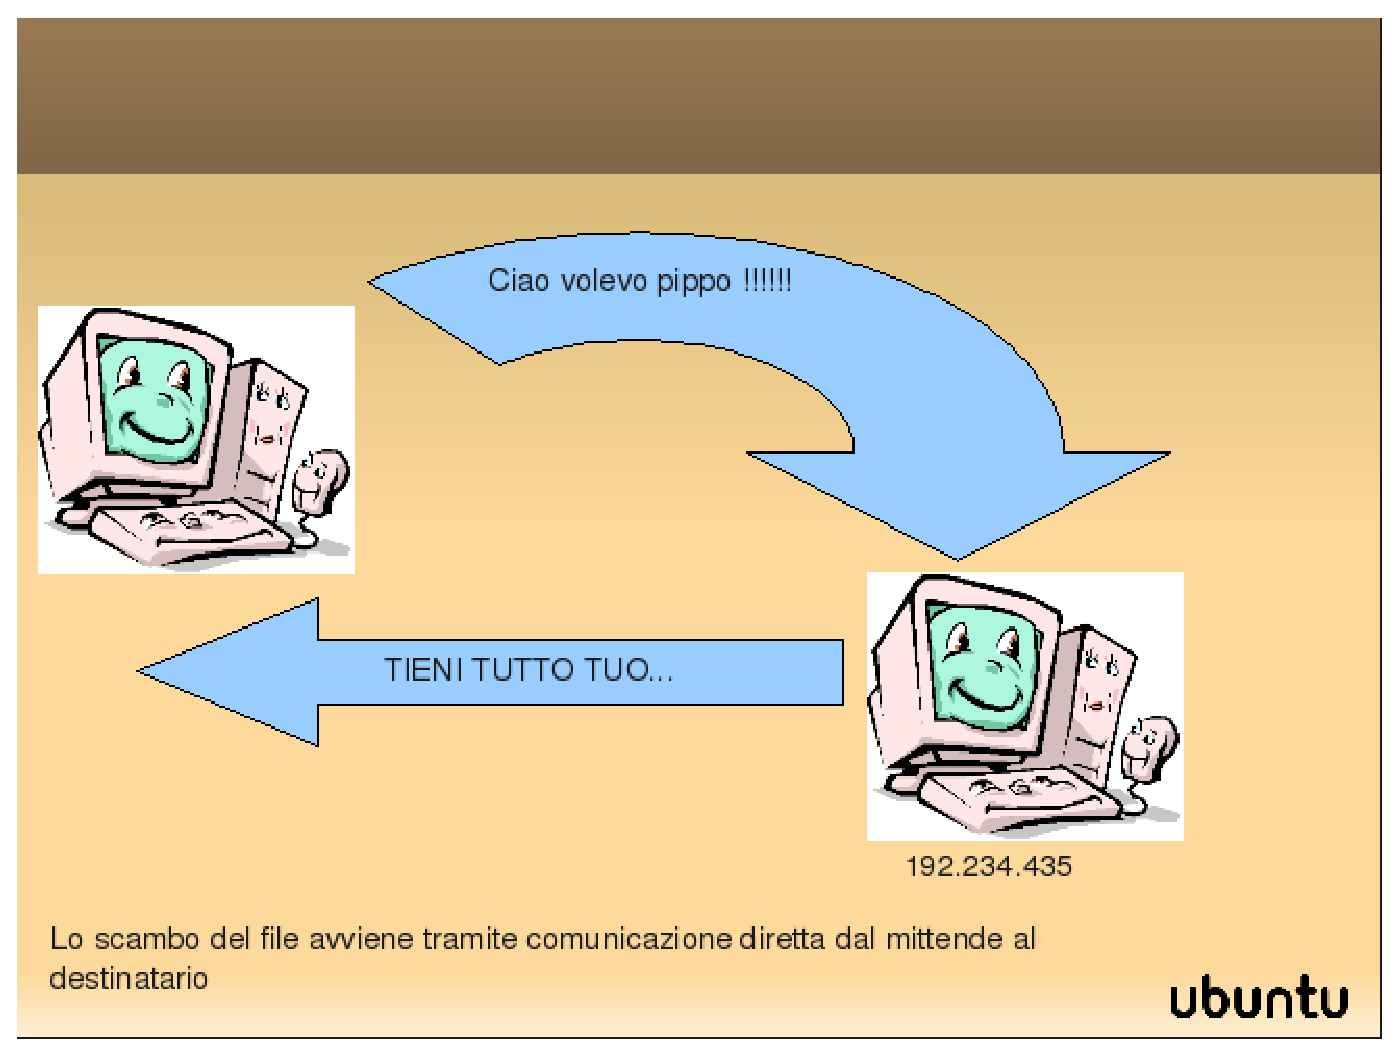
\includegraphics[width=400px,height=375px,bb=14 14 841 737]{images/pluto.eps}
 % mini_kazaa_client.eps: 0x0 pixel, 300dpi, 0.00x0.00 cm, bb=14 14 841 737
 \caption{Download.}
 \label{fig:download}
\end{figure}
%Spiegare perchè mandiamo risposte vuote.

\appendix
\chapter{Manuale d'uso}
Affrontiamo ora la parte piu' pratica del progetto.
\section{Installazione}
Anzitutto e' importante sapere che per poter utilizzare il prodotto da noi creato e' necessaria almeno una rete LAN o una rete INTERNET.
Un computer della rete deve fornire il servizio di bootstrap Server e quindi deve essere avviato come tale.
All'avvio del programma l' utente può decidere se essere un SuperNode o un OrdinaryNode.
Ricordiamo che questa decisione non sarà possibile modificarla nel seguito. 
A seconda della scelta appariranno a video le schermate da utilizzare ed il programma è pronto a funzionare.
\section{Primo avvio}
\begin{figure}[t]
 \centering
 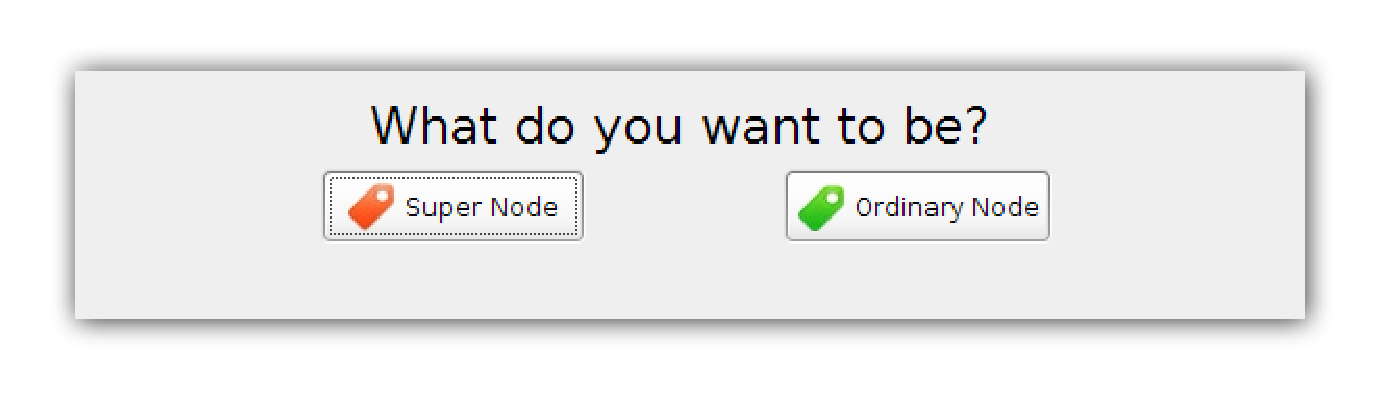
\includegraphics[width=325px,height=75px]{images/what.eps}
 % logica_uml.eps: 0x0 pixel, 300dpi, 0.00x0.00 cm, bb=14 14 593 376
 \caption{Pannello di decisione SuperNode o OrdinaryNode}
 \label{fig:what}
\end{figure}
Per semplicità spieghiamo il primo avvio supponendo di lanciae la nostra applicazione in modalità SuperNode.
Le cose che verranno scritte nella parte sottostante sono analoghe anche se si lanciasse la modalità
OrdinaryNode.
All'avvio appare la schermata mostrata in Figura \ref{fig:what}.
Cliccando sul tasto che corrisponde alla creazione di supernode appare un nuovo pannello mostrato 
in Figura \ref{fig:configuration}.
\begin{figure}[t]
 \centering
 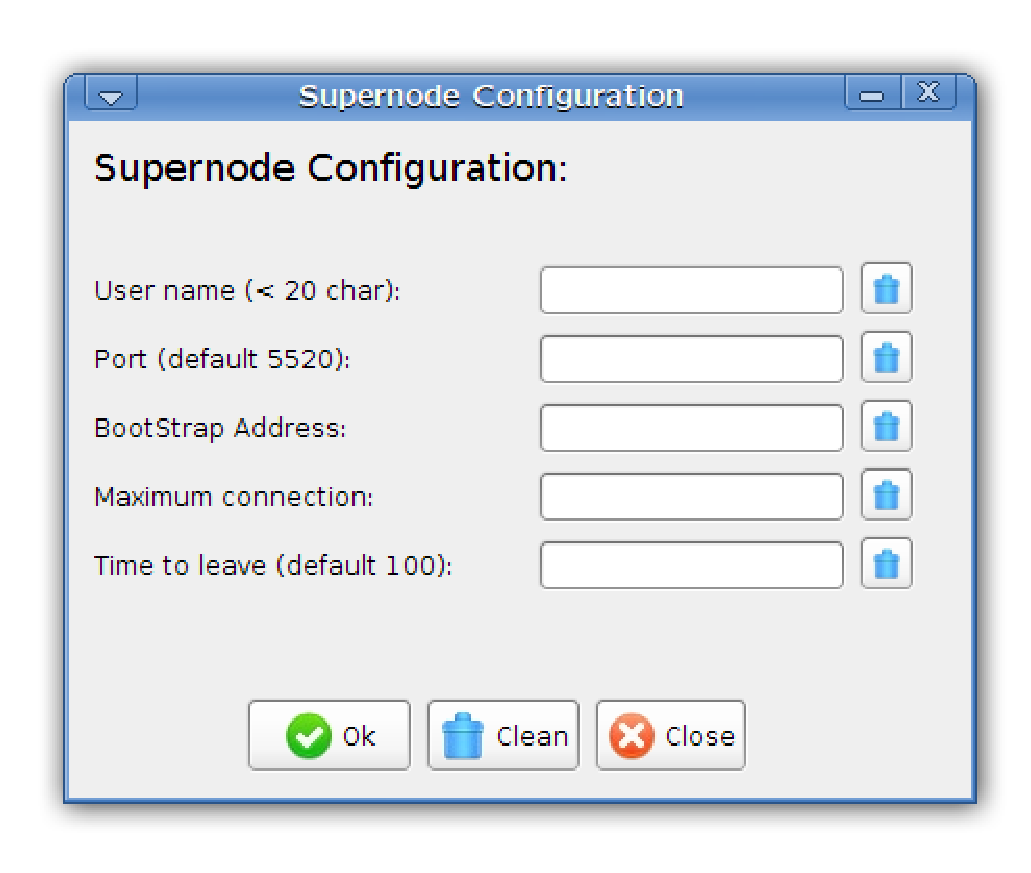
\includegraphics[width=325px,height=200px]{images/configuration.eps}
 % logica_uml.eps: 0x0 pixel, 300dpi, 0.00x0.00 cm, bb=14 14 593 376
 \caption{Il pannello di configurazione del SuperNode.}
 \label{fig:configuration}
\end{figure}
E' necessario ora riempire i campi vuoti per la configurazione del peer.
Inseriamo quindi un nikname che preferiamo, il numero della porta di comunicazione, l' indirizzo del bootstrap server,
il massimo numero di nodi al quale verrà inviata la richiesta di un file ed infine il time to live.
Il settaggio del time to live lo sconsigliamo ad utenti poco esperti dato che potrebbe, se impostato male, rendere l' applicazione
poco funzionante.
Consigliamo inoltre ad utenti esperti che intendano settare il time to live di farlo in modo oculato. 
Per l'applicazione utilizzata su reti di grosse dimensioni è preferibile un time to live maggiore di quello 
impostato di default, mentre al contrario se si lancia l' applicativo su reti di piccola dimensione è preferibile un time to live decisamente 
più piccolo di quello di default.
\begin{figure}[t]
 \centering
 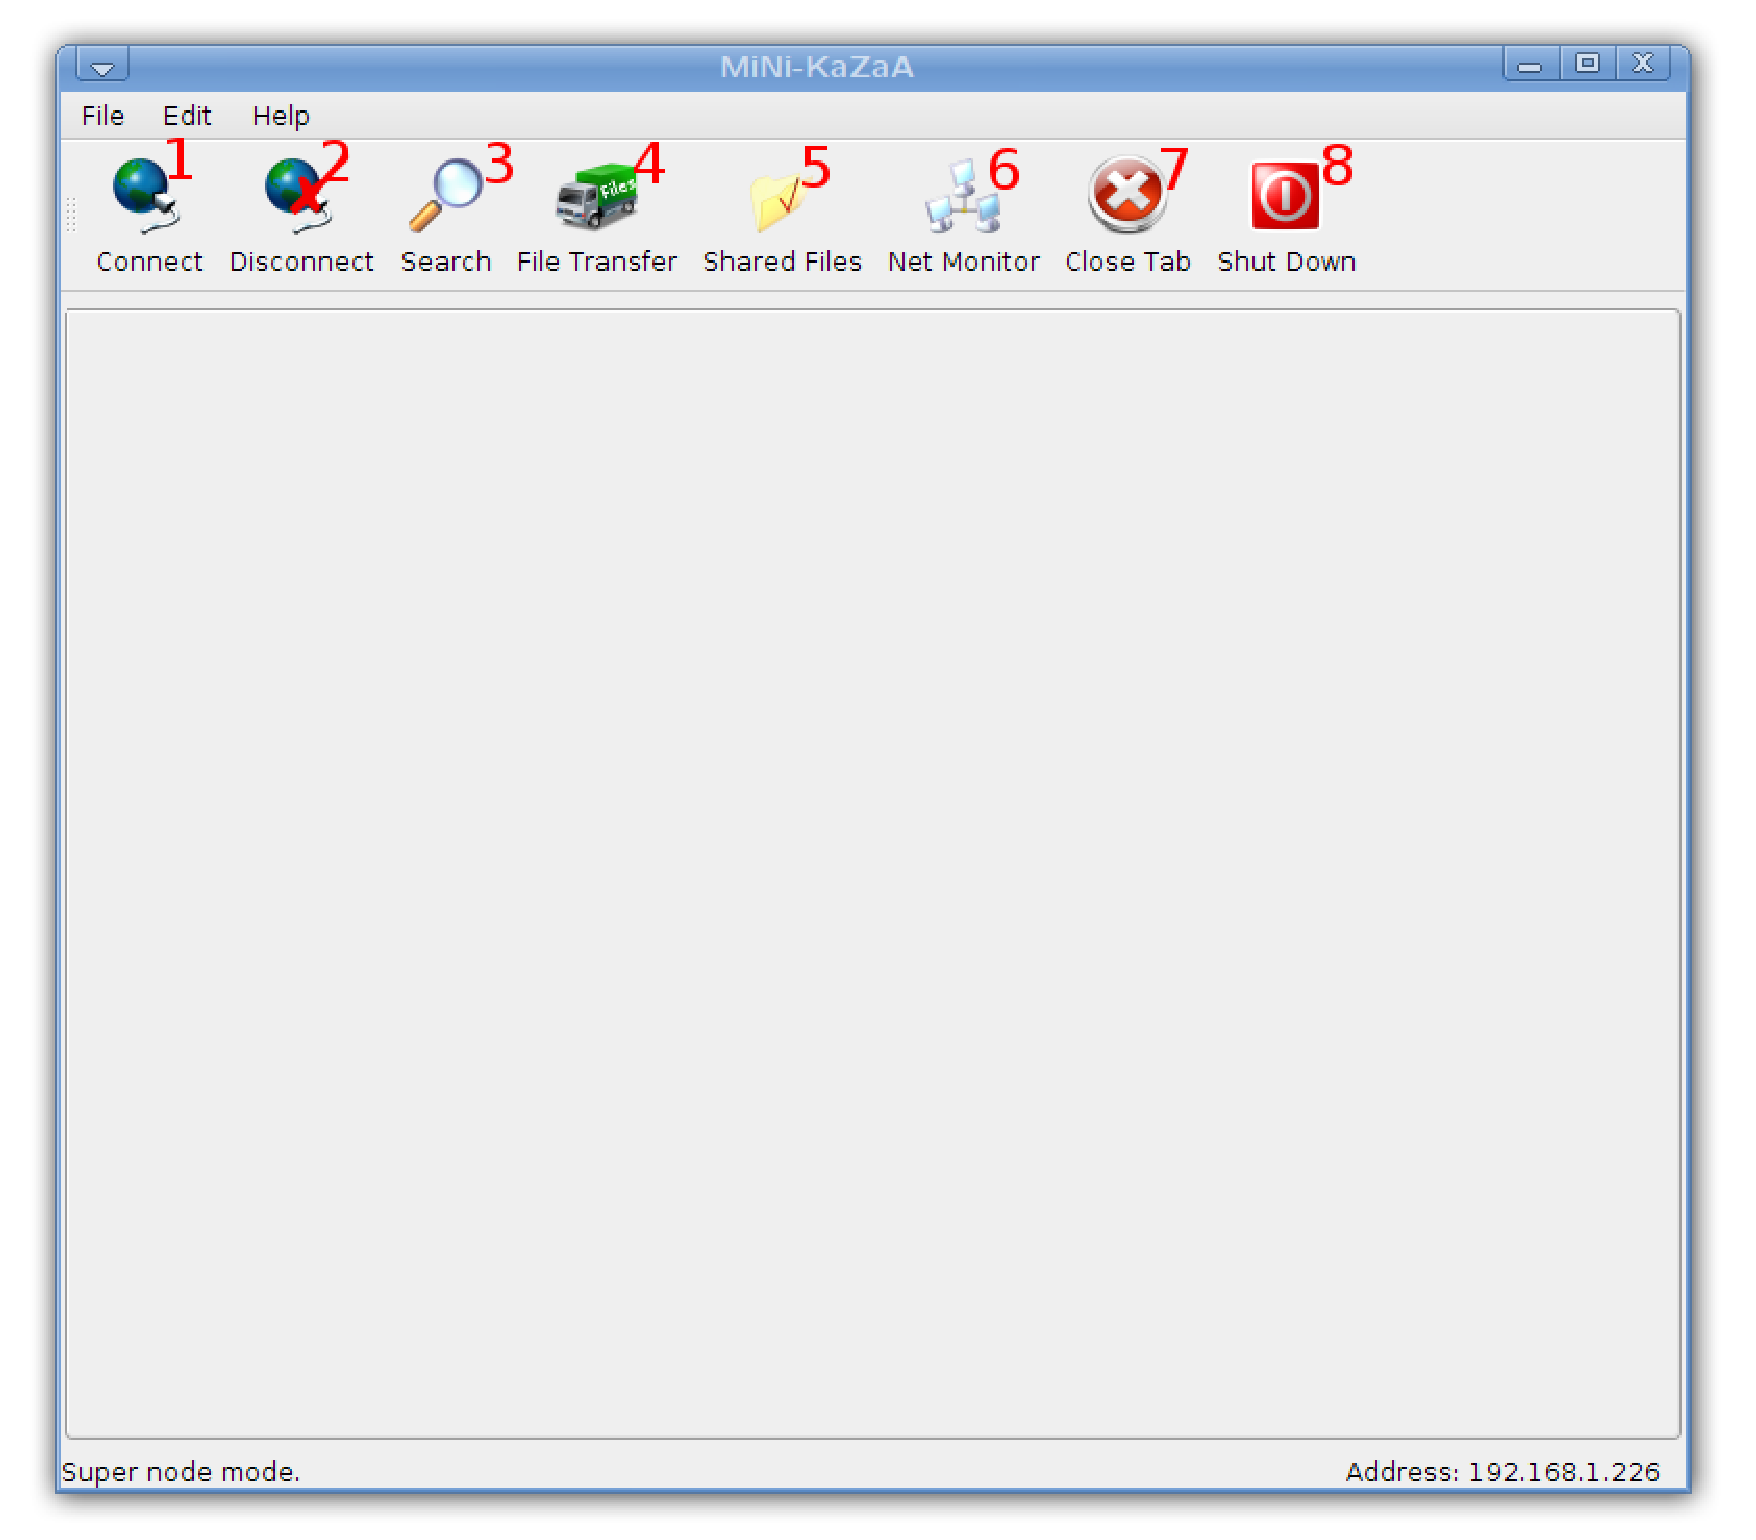
\includegraphics[width=350px,height=225px]{images/mini_kazaa_client.eps}
 % logica_uml.eps: 0x0 pixel, 300dpi, 0.00x0.00 cm, bb=14 14 593 376
 \caption{L' interfaccia principale dell' ordinary node.}
 \label{fig:mini}
\end{figure}
Riempiti tutti i campi correttamente e premuto il tasto ok, se tutto è andato a buon fine apparirà ora la finestra in figura 
\ref{fig:mini}
In caso di campi compilati in maniera non corretta il client provvede a segnalare l'errore con un'apposita \emph{dialog}.
L' installazione è terminata, il programma è funzionanante non vi resta che divertirvi con Mini-KaZaA.

\section{Come funziona}
Bene se siamo di fronte al programma correttamente installato ora non ci rimane che usarlo.
Se abbiamo deciso di essere SuperNode noi vogliamo oltre che poter cercare e scaricare sulla rete fornire il nostro servizio alla comunica globale.
Se abbiamo decido di essere OrdinaryNode noi vogliamo usufruire solamente del servizio di ricerca e download che offre Minikazaa.
	\subsection{Cercare e scaricare un file}
Per cercare e scaricare un file, è necessario inserire nella casella vuota il titolo del file che interessa trovare nella rete.
La nostra casella di ricerca interpreta la parola chiave inserita della casella come una $ *esempio* $ . Questo significa che tutti i file che contengono nel titolo la parola "esempio" verranno restituiti come canditati per lo scaricamento.
Nella tabellina sotto il campo dove è stata inserita la parola ora appariranno i riferimenti ai file che sono presenti sulla rete, i quali possono essere facilmente scaricati cliccando su comodo pulsate download
Il download che parte automaticamente è visibile e controllabile nella sezione chiamata FILETRANSFERT.

	\subsection{Aggiungere un file nella lista dei file condivisi}
Come tutti i servizi di file sharing minikazaa permette di aggiornare la lista dei file che è possibile scaricare.
Cliccando il bottone di Sharing viene caricato automaticamente un pannello che indica la lista dei file che sono stati messi in condivisione nella rete.
E' inoltre possibile aggiungere file alla lista cliccando su tasto add e rimuoverne altri cliccando sul tasto remove.

	\subsection{Controllare lo stato dei download}
Cliccando la sezione FileTranfert si apre un pannello che permette di controllare lo stato dei download dei file che desideriamo scaricare.
Nella tabella che si è appena aperta è possibile vedere il nome del file, la dimensione e il progressivo stato di scaricamento nella barra.

	\subsection{NetMonitor}
Questo tasto risulta disabilitato se avete deciso di essere OrdinaryNode e invece è attivo se avete deciso di essere SuperNode.
Prendiamo ora il caso di essere SuperNode, e di avere aperto il pannello corrispondente a NetMonitor.
Nel suddetto pannello appare la situazione della rete al momento, piu' precisamente la lista dei SuperNode ai quali si è connessi.


	\subsection{Chiudere le schede}
I restanti tasti visibili nella schermata permettono di chiudere le schede aperte in precedenza.

	\section{Consigli degli autori per l' utilizzo}
Al fine di rendere un migliore servizio possibile diamo alcuni consigli per gli utilizzatori del nostro software.
Consigliamo quindi ad utilizzatori dotati di grosse quantità di file, ma soprattutto di grandi capacità di linea di offrire il loro servizio alla comunità globale e quindi di avviare l' applicazione come supernode.
Consigliamo invece agli utenti di piccole dimensione, che hanno difficolta ed un valore di upload limitato di preferire la modalità da ordinaryNode.
  

\end{document}
